\documentclass[oneside, 11pt]{article}

\usepackage[T1]{fontenc}
\usepackage[utf8]{inputenc}
\usepackage[dutch]{babel}

\usepackage{fouriernc}
\usepackage[detect-all, load-configurations=binary,
            separate-uncertainty=true, per-mode=symbol,
            retain-explicit-plus, range-phrase={ tot }]{siunitx}

\usepackage{setspace}
\setstretch{1.2}

\setlength{\parskip}{\smallskipamount}
\setlength{\parindent}{0pt}

\usepackage{geometry}
\geometry{marginparwidth=0.5cm, verbose, a4paper, tmargin=3cm, bmargin=3cm, lmargin=2cm, rmargin=2cm}

\usepackage{float}

\usepackage[fleqn]{amsmath}
\numberwithin{equation}{section}
\numberwithin{figure}{section}

\usepackage{graphicx}
\graphicspath{{Figures/}}
\usepackage{subfig}

\usepackage{tikz}
\usetikzlibrary{plotmarks}

\usepackage{fancyhdr}
\pagestyle{fancy}
\fancyhf{}
\rhead{\thepage}
\renewcommand{\footrulewidth}{0pt}
\renewcommand{\headrulewidth}{0pt}

\usepackage{relsize}
\usepackage{xspace}
\usepackage{url}

\newcommand{\figref}[1]{Figuur~\ref{#1}}

\newcommand{\hisparc}{\textsmaller{HiSPARC}\xspace}
\newcommand{\kascade}{\textsmaller{KASCADE}\xspace}
\newcommand{\sapphire}{\textsmaller{SAPPHiRE}\xspace}
\newcommand{\jsparc}{\textsmaller{jSparc}\xspace}
\newcommand{\hdf}{\textsmaller{HDF5}\xspace}
\newcommand{\aires}{\textsmaller{AIRES}\xspace}
\newcommand{\csv}{\textsmaller{CSV}\xspace}
\newcommand{\python}{\textsmaller{PYTHON}\xspace}
\newcommand{\corsika}{\textsmaller{CORSIKA}\xspace}
\newcommand{\labview}{\textsmaller{LabVIEW}\xspace}
\newcommand{\daq}{\textsmaller{DAQ}\xspace}
\newcommand{\adc}{\textsmaller{ADC}\xspace}
\newcommand{\adcs}{\textsmaller{ADC}s\xspace}
\newcommand{\Adcs}{A\textsmaller{DC}s\xspace}
\newcommand{\hi}{\textsc{h i}\xspace}
\newcommand{\hii}{\textsc{h ii}\xspace}
\newcommand{\mip}{\textsmaller{MIP}\xspace}
\newcommand{\hisparcii}{\textsmaller{HiSPARC II}\xspace}
\newcommand{\hisparciii}{\textsmaller{HiSPARC III}\xspace}
\newcommand{\pmt}{\textsmaller{PMT}\xspace}
\newcommand{\pmts}{\textsmaller{PMT}s\xspace}

\DeclareSIUnit{\electronvolt}{\ensuremath{\mathrm{e\!\!\:V}}}

\DeclareSIUnit{\unitsigma}{\ensuremath{\sigma}}
\DeclareSIUnit{\mip}{\textsmaller{MIP}}
\DeclareSIUnit{\adc}{\textsmaller{ADC}}

\DeclareSIUnit{\gauss}{G}
\DeclareSIUnit{\parsec}{pc}
\DeclareSIUnit{\year}{yr}



\title{Analyse met Coach}
\author{C.G.N. van Veen}
\docanalyse{4}{AC}
\version{1.1}

\begin{document}

\maketitle

\section{Inleiding}

Dit werkblad helpt leerlingen en docenten om data analyse van \hisparc met 
het software pakket Coach (6 of 7) te doen. Coach (6 of 7) is een software pakket wat leerlingen
en docenten in staat stelt om fysische grootheden te meten en analyses met deze 
data te doen. Coach is al op veel scholen beschikbaar en leerlingen kunnen hier
gemakkelijk mee aan de slag.
We gebruiken het onderdeel `analyse' van Coach om ESD data van \hisparc te analyseren.
In dit document wordt stap voor stap uitgelegd hoe je deze data in kunt laden in 
Coach. Daarnaast wordt uitgelegd hoe je van deze data in Coach
grafieken kunt plotten en analyseren. In dit document wordt eerst uitgelegd hoe
dit met Coach6 gedaan wordt. Het laatste deel van dit document licht toe hoe dezelfde grafieken
in Coach7 gemaakt worden.

\section{Het ophalen van ESD data}

Ga naar de volgende website http://data.hisparc.nl en kies een station waar 
je data van wilt downloaden. Klik op het station, je gaat nu naar een andere site.
Kies nu op deze site de link aan de rechterkant: `Download event summary data'.
In `Info Pakket' kun je in het bestand `data retrieval' precies te zien hoe je 
nu de data als een excel bestand kunt downloaden.
Kies voor het gemak voor één dag data, dan is het bestand nog redelijk klein.
Je krijgt een csv-bestand binnen waarin als eerste (de eerste 28 regels) beschreven staat wat je 
in elke kolom aan data vindt. In het csv-bestand vindt je onder andere, tijdstempel per event,
pulshoogte en pulsintegraal per detector, aantal deeltjes per detector en aankomsttijden van
de shower in de detector.

\section{Inlezen van de data in Coach.}

Het csv bestand gaan we nu inlezen in Coach. Open Coach; log in als docent; kies `nieuwe activiteit'; 
`meten'. (Je hoeft geen meetpaneel te kiezen.)

Klik op het icoon tabel, zie \figref{fig:coach1}. Je kunt hier kiezen om een
nieuwe tabel aan te maken. Er verschijnt een werkvenster `tabel kiezen of maken'.
Kies in dit werkvenster `importeren'. In het uitklapvenster kies je 'tekst bestand'.

\textit{Deel van de HiSPARC data uit een .csv bestand.}
\begin{verbatim}
15/07/15	14:00:10	1436968810	060318189     4	    6	256	  122	0	...	
15/07/15	14:00:13	1436968813	006833767  1416	  485	255	 1041 0 ...
15/07/15	14:00:13	1436968813	116782974     4	  351	272	    6	0	...
15/07/15	14:00:13	1436968813	344642048     6	  379	261	    4	0	...	
15/07/15	14:00:14	1436968814	113137182     5	    5	223	  136	0	...	
15/07/15	14:00:20	1436968820	261698618     4	  247	  4	  365	0	...
\end{verbatim}

\begin{figure}
    \centering
    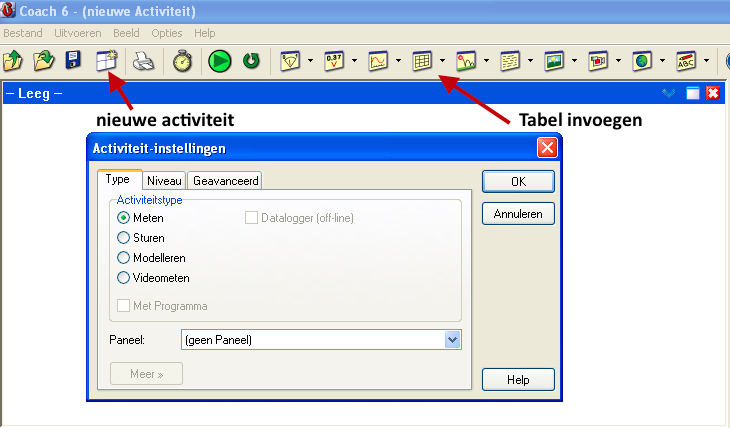
\includegraphics[scale=0.6]{coach1}
    \caption{Screenshot van coach 6, open een nieuwe activiteit door op 
    het icoon linksboven te klikken (vier window icoon).In de nieuwe activiteit 
    "meten" kun je nu een tabel invoegen. Het icoon van tabel invoegen is 
    aangegeven met de rechterpijl. Klik op dit icoon, er verschijnt dan een werkvenster.}
    \label{fig:coach1}
\end{figure}

\begin{figure}
    \centering
    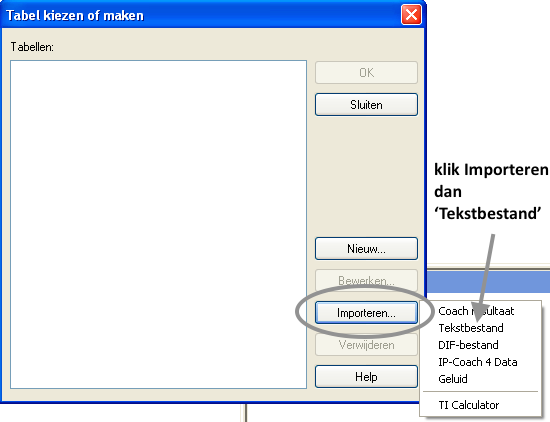
\includegraphics[scale=0.6]{coach2}
    \caption{Importeren van een csv-bestand met Coach. Kies tabel `importeren' en
    dan `tekstbestand'.}
    \label{fig:coach2}
\end{figure}

Bij het importeren van het .csv bestand moet je aangeven hoe Coach het bestand moet 
lezen. In \figref{fig:coach3} kun je zien dat je dat het decimaal teken
een punt moet zijn. Voor duizendtallen mag je ook `geen' invullen. Omdat je de tekst
boven de data in het csv bestand niet wilt, moet je aangeven dat je vanaf rij 
28 begint.

\begin{figure}
    \centering
    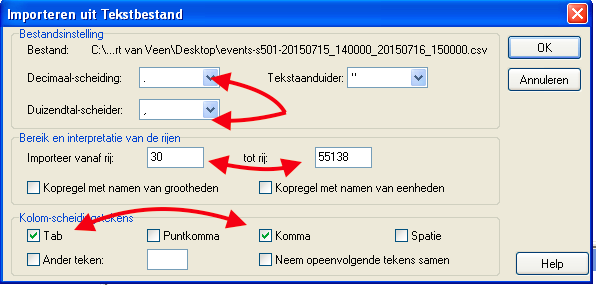
\includegraphics[scale=0.6]{coach3}
    \caption{Instellen van importeer mogelijkheden in Coach.}
    \label{fig:coach3}
\end{figure}
   
Als je nu op `ok' klikt ben je bijna klaar met importeren. Je kunt nu boven elke
kolom aangeven wat er voor data in staat. De eerste twee kolommen bevatten in Coach 6 
helaas niets, omdat datum en tijd niet herkend worden. De kolommen 3 tot en met 
8 bevatten wel data die we kunnen gebruiken. In kolom 3 staat het GPS-tijdstempel UNIX epoch.
Dat betekent dat we datum-tijdstempel van het event in het aantal seconden na 1 januari 1970 uitdrukken.
Kolom 4 heeft het tijdstempel in het aantal nanoseconden.
Kolommen 5 tot en met 8 bevatten de pulshoogte waarden voor een bepaald event.
Je kunt het aantal decimalen instellen op 0 voor elke grootheid. Zie \figref{fig:coach4} 

Klik nu `ok'. Nu is de data van het .csv bestand als tabel 1 beschikbaar.
klik op tabel 1 en plaats deze in een venster.

\begin{figure}
    \centering
    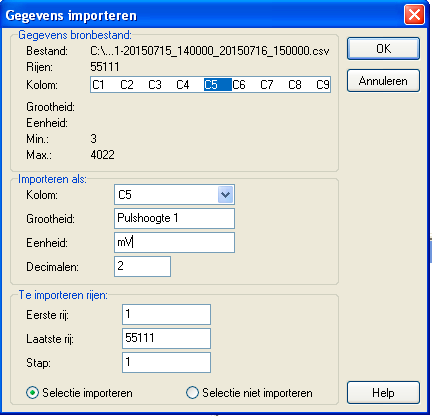
\includegraphics[scale=0.6]{coach4}
    \caption{Kolommen de juiste naam geven.}
    \label{fig:coach4}
\end{figure}


\section{Pulshoogte diagram in Coach}

We hebben nu de data van het .csv bestand ingelezen in Coach en gaan er een
pulshoogte histogram van plotten. Daarna kunnen we met behulp van de analyse 
mogelijkheden in Coach kunnen we onderzoek doen aan het histogram.

\subsection{Pulshoogte diagram maken}

De snelste manier om een histogram is om op de betreffende kolom in het tabel venster
'rechts' te klikken en dan uit het analyse menu, histogram te kiezen.
Je moet echter aangeven in hoeveel stappen je het histogram wilt laten maken.
Dan geef je aan bij 'aantal klassen'. Verander dit bijvoorbeeld in 200. Onderzoek
ook het effect van meer of minder `klassen' (in het Engels wordt dit het aantal 
`Bins' genoemd.)

\begin{figure}
    \centering
    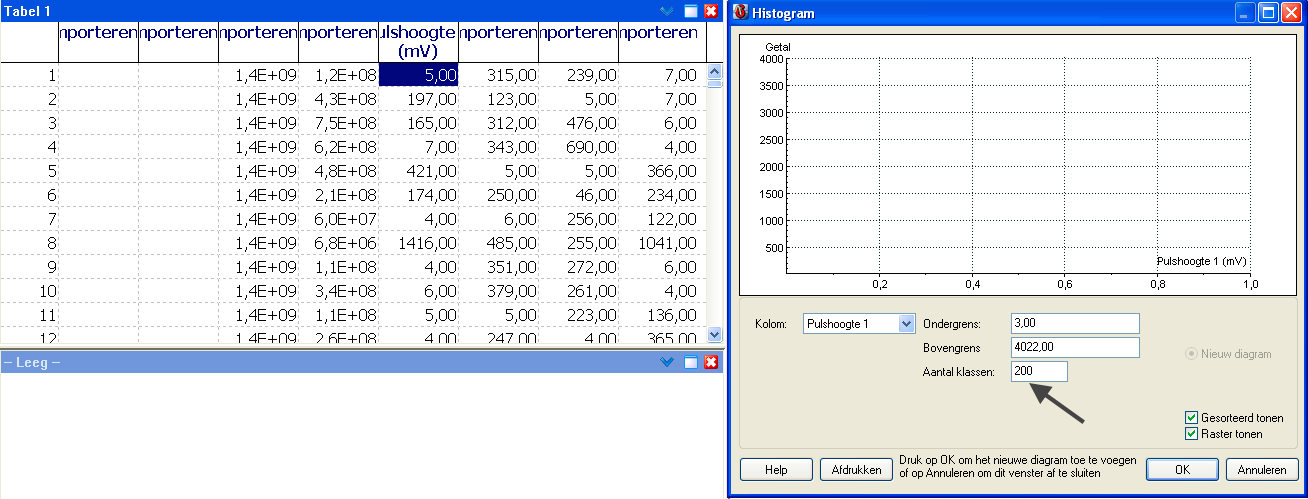
\includegraphics[scale=0.4]{coach5}
    \caption{Aantal klassen aanpassen voor het histogram.}
    \label{fig:coach5}
\end{figure}

Klik `ok' en plaats het diagram in een leeg window. Kies nu 'automatisch zoomen'.
Nu zie je een histogram van de pulshoogte van detector 1.

\textbf{Opdracht 1.}
Maak nog 3 dezelfde histogrammen van de andere detectoren. Plaats deze apart in diagrammen.
(je kunt zo ook in een diagram plaatsen.)

We willen graag een logaritmische y-as, dat kunnen we instellen.
Klik rechts op het diagram, kies `diagram instelling'. Zie \figref{fig:coach6}
Zorg dat je kolom C3 onzichtbaar maakt (tip: geef C3 een duidelijke naam bij het vakje
grootheid). In C4 maak je een formule, selecteer C4 en kies de formule knop. 
Maak nu een formule waarin je de log van de grootheid van C3 neemt. 
In 'diagram instelling' kun je ook nog aangeven welke kleur de grafiek moet hebben en
of je de meetwaarden als stip of als kruis wilt zien. In \figref{fig:coach7} zie je 
de grafieken. Een grafiek met en één grafiek zonder logaritmische schaal.


\begin{figure}
    \centering
    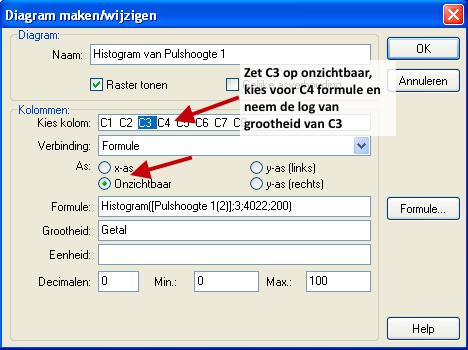
\includegraphics[scale=0.6]{coach6}
    \caption{Instellingen voor het logaritmische pulshoogte diagram.}
    \label{fig:coach6}
\end{figure}

\begin{figure}
    \centering
    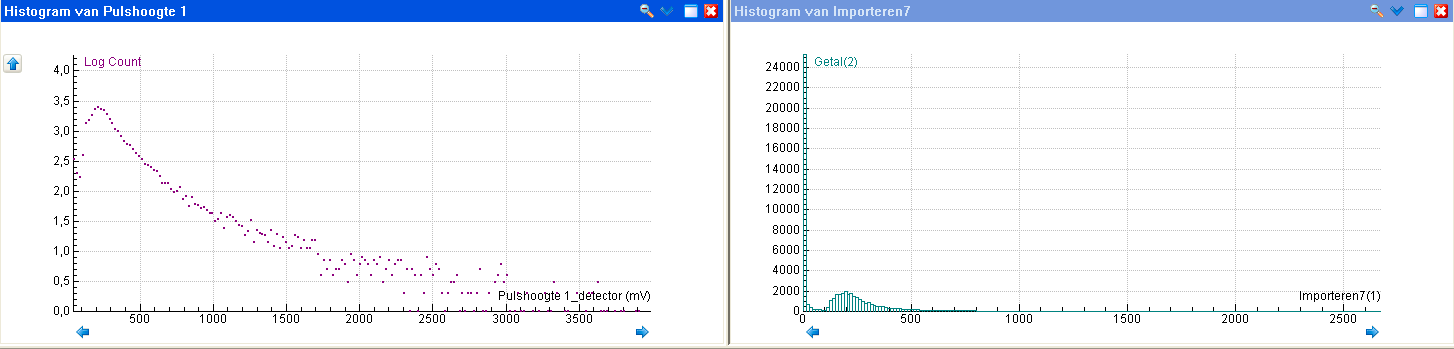
\includegraphics[scale=0.3]{coach7}
    \caption{Pulshoogte diagrammen, lineair en logaritmisch}
    \label{fig:coach7}
\end{figure}
 
 
\subsection{opdrachten} 
\label{sec:opdrachten}

\textbf{Opdracht 1.}
Maak nog 3 dezelfde histogrammen van de andere detectoren. Plaats deze apart in diagrammen.
(je kunt ook twee grafieken in één diagram plaatsen.)

\textbf{Opdracht 2.}
Gebruik de analyse of uitlees optie om de waarde van de piek in de diagrammen
uit te lezen. Noteer deze. Zijn ze voor elke detector precies hetzelfde?

\textbf{Opdracht 3.}
Analyseer de helling van het logaritmische diagram. Gebruik de 'analyse' en dan 'helling'
mogelijkheid, die je vindt door rechts te klikken op het diagram. 
Teken op een afstand van 3x de waarde van de piek die je bij opdracht 2 vond een beste raaklijn aan de
grafiek. Zie \figref{fig:coach8}. Klik in het analyse venster op het punt en verander
de helling van de raaklijn met de pijltjes toetsen.

\textbf{Opdracht 4.}
a.
Download een csv bestand met weerdata van de \hisparc website.
Kies dan een \hisparc station wat ook een weerstation heeft.
Maak eens wat plotjes van bijvoorbeeld de luchtdruk, windsnelheid,temperatuur,
tegen het tijdsverloop over een dag.

b. Bepaal met een histogram van de pulshoogte piek van een warme zomerdag of 
een winterdag. Zie je verschillen. 

\begin{figure}
    \centering
    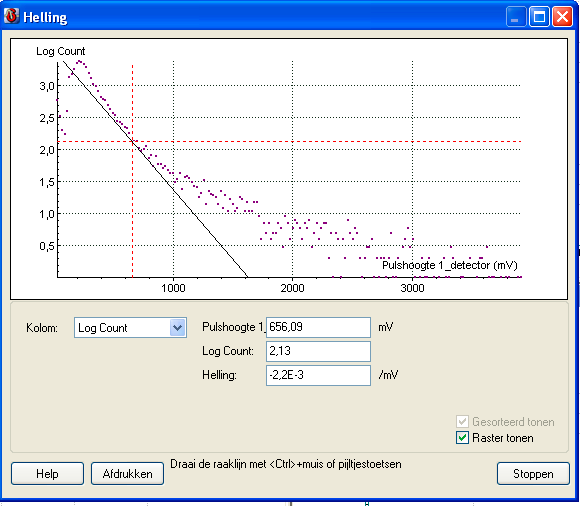
\includegraphics[scale=0.4]{coach8}
    \caption{Bepaling van de helling van het pulshoogte diagram op een afstand
    van 3x de piek waarde.}
    \label{fig:coach8}
\end{figure}

\section{Werken met Coach7}

De nieuwe versie van Coach (7), maakt het mogelijk om meer dan acht kolommen in te lezen
uit een gedownload csv bestand. In ons geval worden zelfs alle 21 kolommen van een event in gelezen.
Omdat Coach7 een ander uiterlijk en andere symbolen voor de knoppen heeft, wordt 
in deze sectie aandacht besteed aan het doen van analyse op de gegevens met Coach7.

In \figref{fig:coach9} is een screenshot van Coach7 te zien. Er is gebruikt gemaakt van een Engelse versie van 
Coach7. Login als `Author' en kies voor activity type `Measurement'.

\begin{figure}
    \centering
    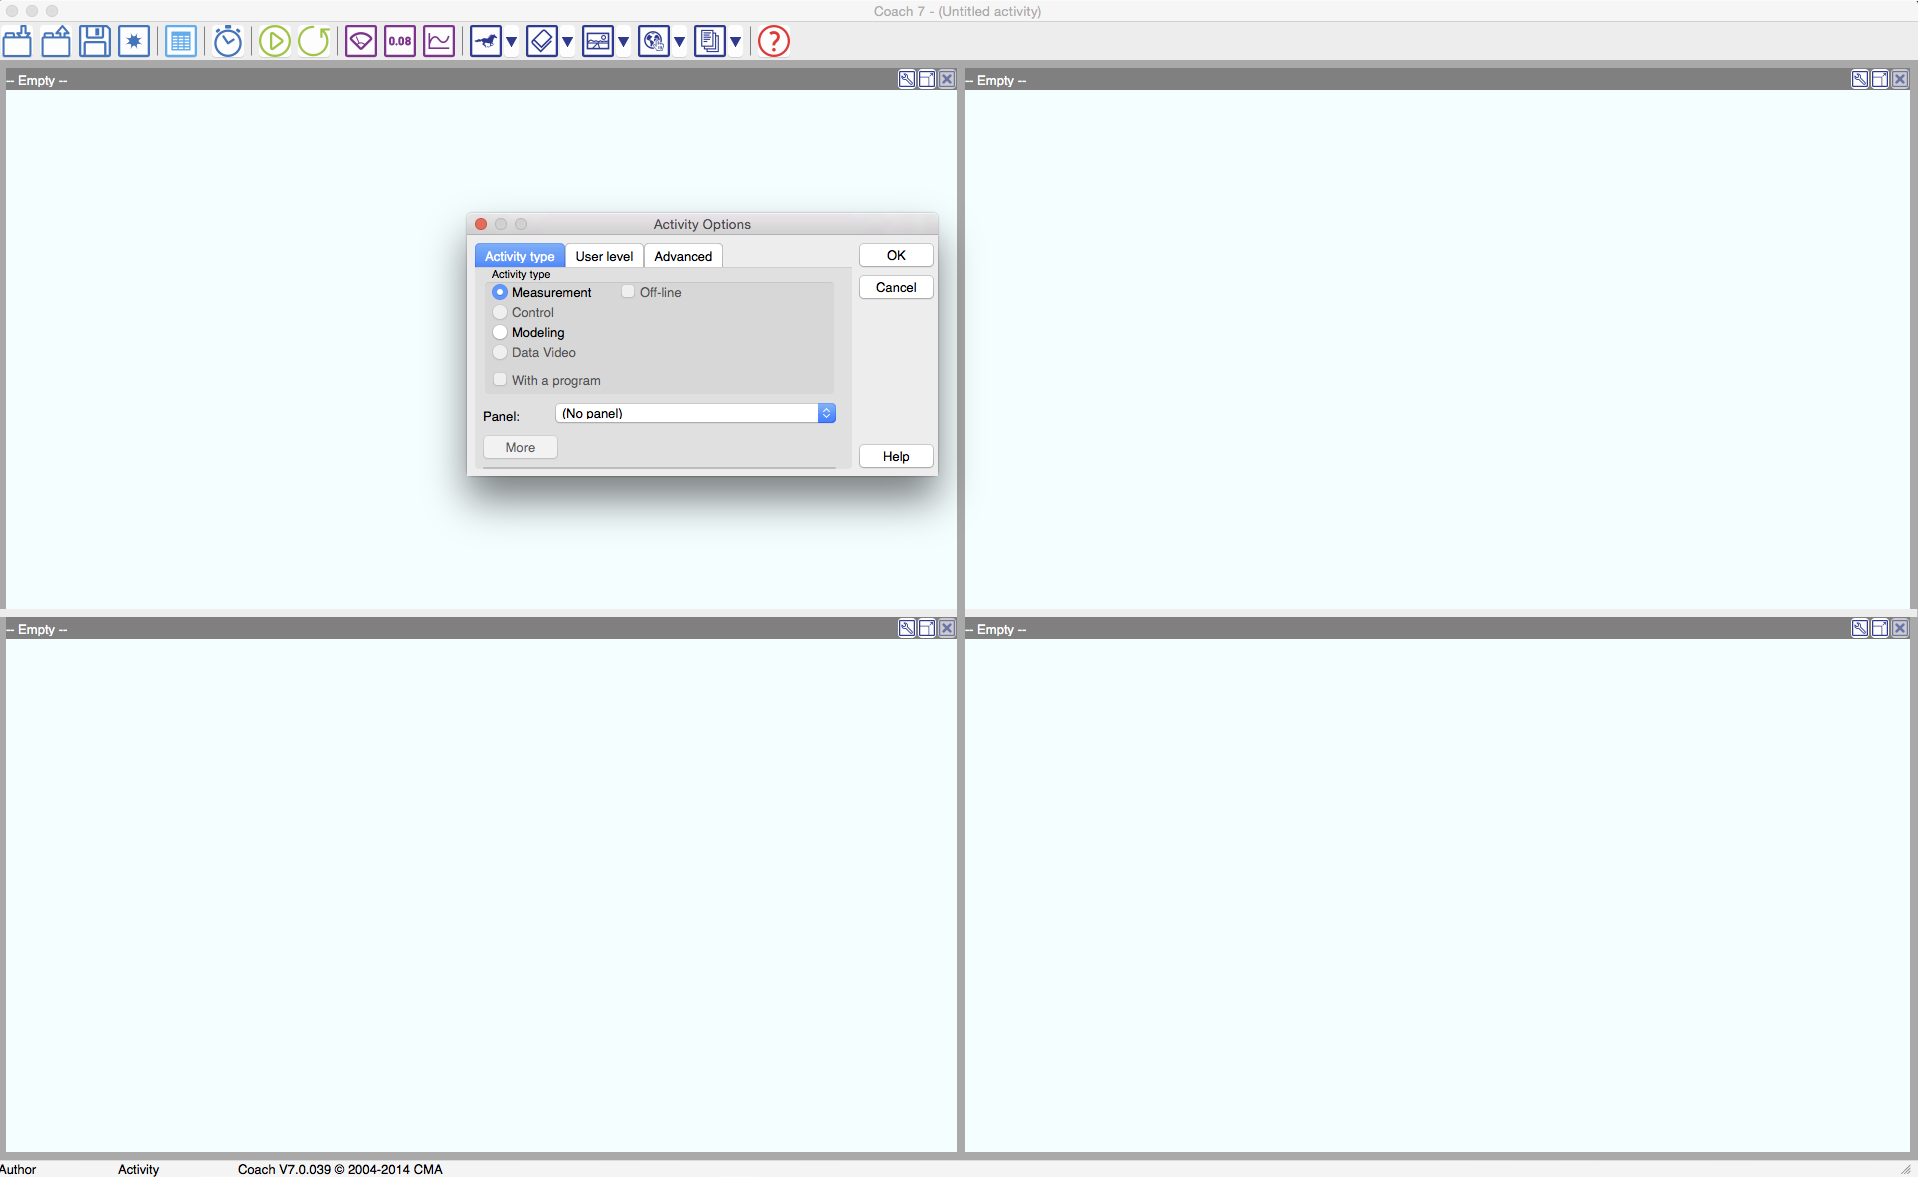
\includegraphics[scale=0.2]{coach9}
    \caption{Screenshot van het openingsscherm van Coach7}
    \label{fig:coach9}
\end{figure}

Nu we in de activiteit omgeving zitten kunnen we het .csv bestand importeren.
Klik op het tabel icoon. Nu opent een tabel venster.
Als je met een rechtermuisknop op het scherm in het tabel venster klikt, verschijnt 
een uitklapmenu waarin je aangeeft bij runs, import, dat je een textfile wilt importeren. 
Zie \figref{fig:coach10}

\begin{figure}
    \centering
    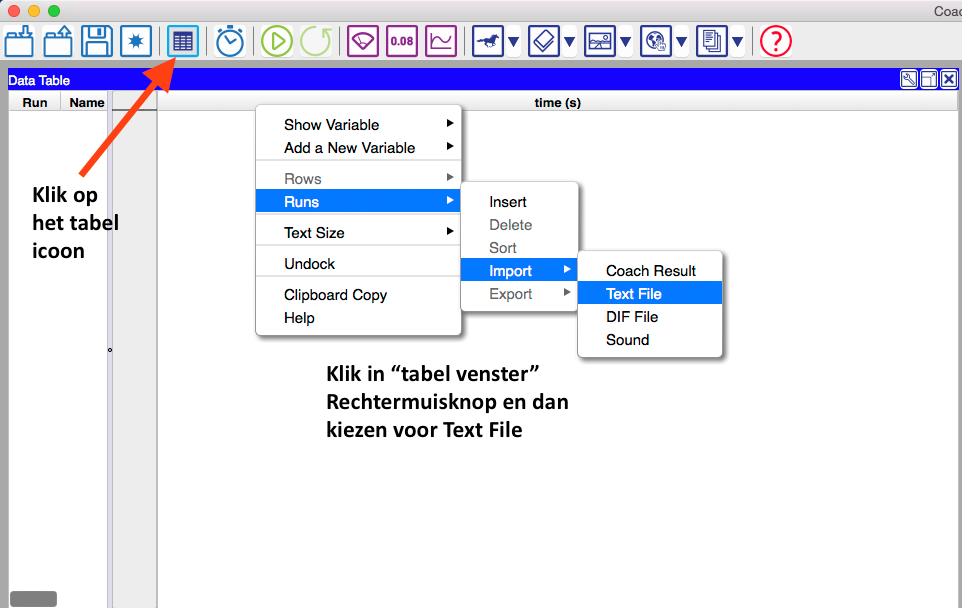
\includegraphics[scale=0.4]{coach10}
    \caption{Importeren van een .csv bestand.}
    \label{fig:coach10}
\end{figure}

Na het selecteren van het juiste .csv bestand krijgen we een soortgelijk scherm
als in figuur \ref{fig:coach3}. In \figref{fig:coach11} zien we ook deze instellingen.
Na het instellen van dit venster klikken we `ok'.

\begin{figure}
    \centering
    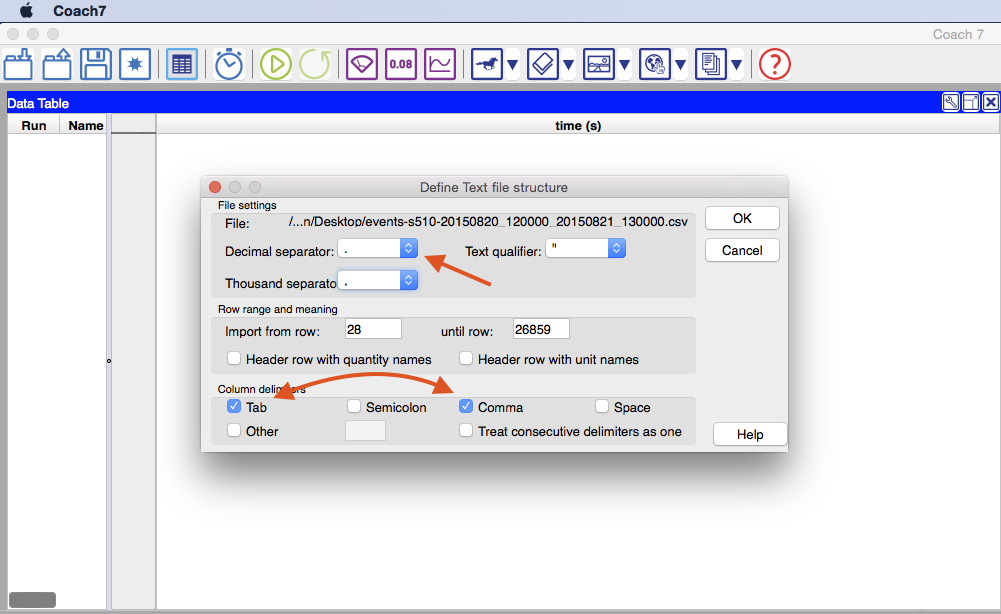
\includegraphics[scale=0.4]{coach11}
    \caption{Instellen voor het importeren van data.}
    \label{fig:coach11}
\end{figure}

\begin{figure}
    \centering
    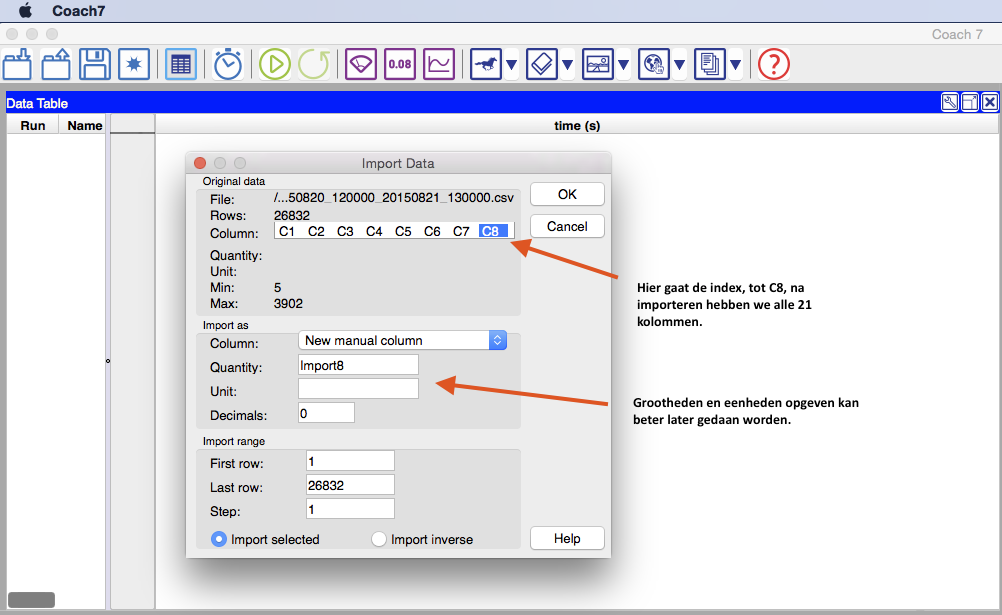
\includegraphics[scale=0.4]{coach12}
    \caption{In dit menu hoeven we niets te veranderen.}
    \label{fig:coach12}
\end{figure}

Nu we alle data geïmporteerd hebben krijgen we de waarden in een tabel. Klik op het plusje
linksboven in het tabel venster, om de tabel uit te klappen.
Nu zien we alle kolommen die geïmporteerd zijn. We kunnen nu dubbelklikken op 
de tekst boven een kolom. Dan opent een menu waarin we de namen van grootheden en eenheden
kunnen aanpassen. Zie \figref{fig:coach13}.  

\begin{figure}
    \centering
    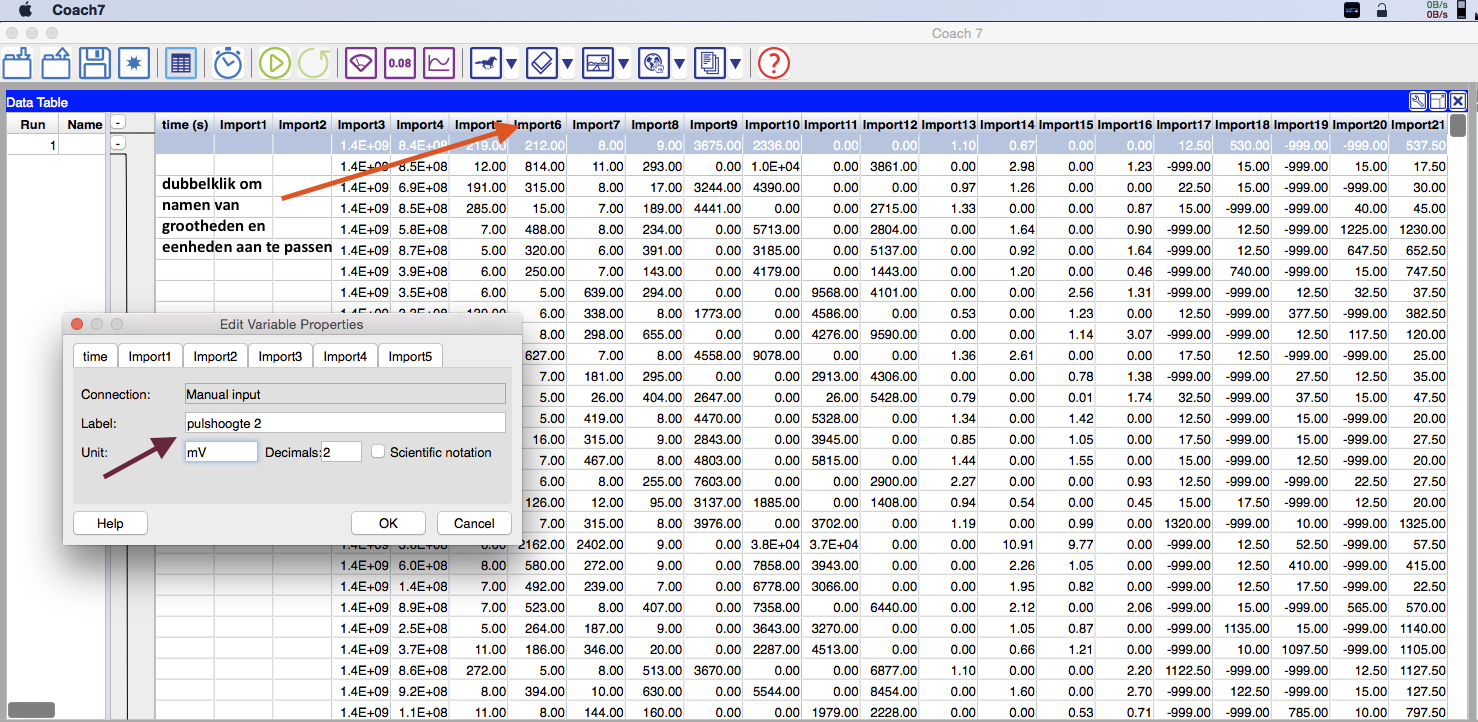
\includegraphics[scale=0.2]{coach13}
    \caption{Dubbelklik de kolomkop en pas daarna de grootheden en eenheden 
    van de gewenste kolommen aan.}
    \label{fig:coach13}
\end{figure}

Klik nu op een leeg venster en kies `weergeven als grafiek'. Er verschijnt dan een
uitklap menu waarin je kunt aangeven welke kolom je grafisch wilt zien. 
Kies de gewenste kolom. Er wordt eerst een standaard index grafiek gemaakt, die 
we aanpassen door het gereedschapskistje boven in het grafiek venster te kiezen. 
Uit het menu van het analyse gereedschapskistje kies je `histogram'. Er wordt 
nu een histogram (pas weer het aantal klassen aan) gemaakt. De volgende stappen 
om uiteindelijk op een logaritmisch histogram te komen zijn identiek aan het 
werken met Coach6.
\hspace{3 mm}

\textbf{Opdracht 5.}
Probeer de opdrachten van paragraaf \ref{sec:opdrachten} nu met Coach7 te doen.

\begin{figure}
    \centering
    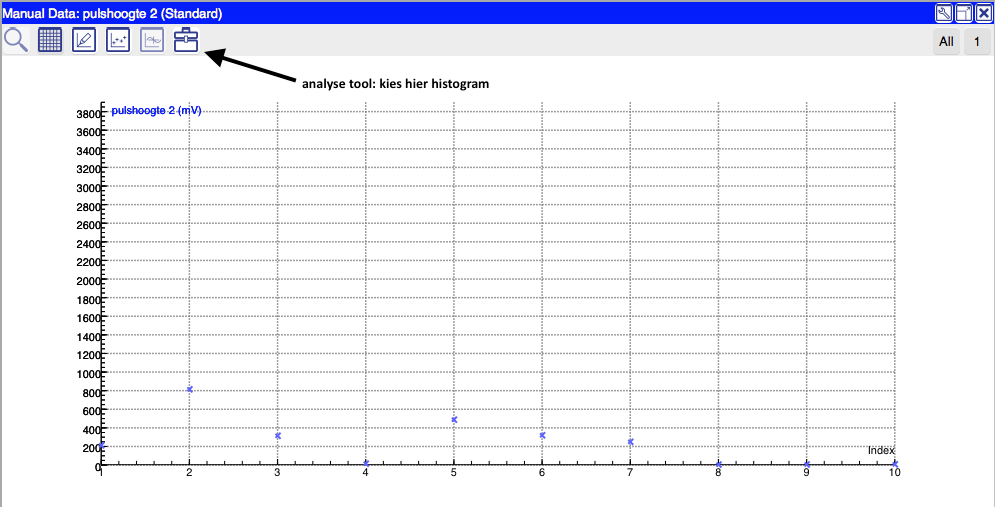
\includegraphics[scale=0.4]{coach14}
    \caption{Klik op de gereedschapskist (het analyse menu verschijnt). Kies `Histogram'.}
    \label{fig:coach14}
\end{figure}

\end{document}
